%!TEX program = xelatex

\documentclass[12pt]{article}
\usepackage[UTF8]{ctex}
\usepackage{indentfirst}
\usepackage{lmodern}
\usepackage{setspace}
\usepackage{verbatim}
\usepackage{amsmath}
\usepackage{amsthm}
\usepackage{graphicx}
\usepackage{subfigure}
\usepackage{booktabs}
\usepackage{tabularx}
\usepackage{multirow}
\usepackage{multicol}
\usepackage{listings}
\usepackage{relsize}
\usepackage[usenames]{color}   
\usepackage{fontspec}
\usepackage{geometry}
\geometry{left=2.0cm,right=2.0cm,top=2.5cm,bottom=2.5cm}
\usepackage{enumitem}
\setlist[enumerate]{listparindent=\parindent}
\usepackage[table]{xcolor}
\usepackage{array}
\usepackage[rightcaption]{sidecap}
\usepackage{hyperref}
\usepackage{float}
\usepackage{tikz}
\usetikzlibrary{shapes.geometric, arrows, positioning}

\hypersetup{
	colorlinks=true,
	linkcolor=black
}
\lstset{
 columns=fixed,       
 numbers=left,                                        
 numberstyle=\tiny\color{gray},                       
 frame=none,                                          
 backgroundcolor=\color[RGB]{245,245,244},            
 keywordstyle=\color[RGB]{40,40,255},                 
 commentstyle=\it\color[RGB]{0,96,96},                
 stringstyle=\rmfamily\slshape\color[RGB]{128,0,0},   
 showstringspaces=false,                              
 breaklines=true,                                     
 language=python,                                     
}
\newcommand{\myd}{\;\mathrm{d}}
\renewcommand{\arraystretch}{1.8}
\renewcommand\refname{参考网站}

\setlength{\parindent}{2em}
\addtolength{\parskip}{3pt}
\onehalfspacing 
\graphicspath{{./figures/}} 
\newcommand{\daima}[1]{{\ttfamily{#1}}}

\setlist[itemize]{itemsep=-4pt}
\setlist[enumerate]{itemsep=-4pt}

\newcolumntype{H}{>{\centering\arraybackslash}p{2cm}}
\newcolumntype{C}{>{\centering\arraybackslash}p{2.4cm}}

\usepackage{algorithm2e}
\usepackage{amssymb}
\begin{document}
\begin{titlepage}
	\vspace*{-2.5cm}
	\begin{figure}[h]
		\centering
		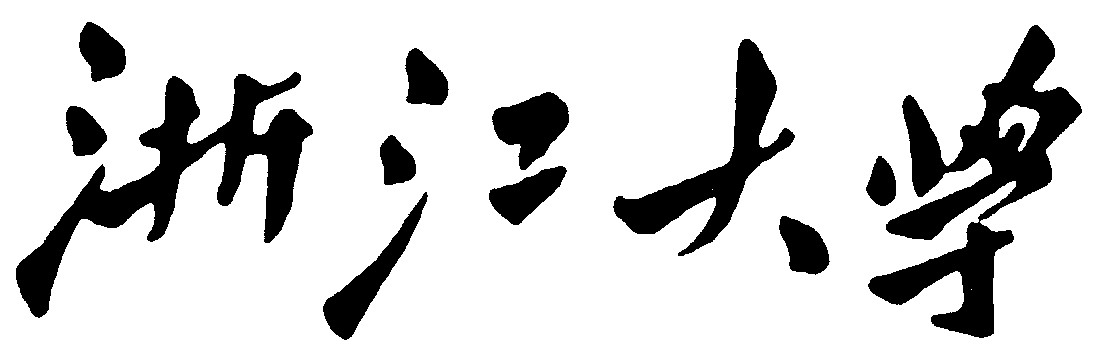
\includegraphics[width=0.8\linewidth]{zjdx}
	\end{figure}
	\begin{figure}[h]
		\centering
		
\includegraphics[width=0.3\linewidth]{qsy}
	\end{figure}
	\vspace{-0.2cm}
	\begin{center}
		\Huge{\textbf{用于广播碰撞域的新型通信协议设计：CSMA/DCR}}\\
	\end{center}
	\vspace*{0.8cm}
	\begin{center}
		\larger[2]{
			\begin{tabular}{cc}
				姓\hspace{12pt}名 & \underline{\makebox[220pt]{\kaishu 黄鹤翔}}             \\
				学\hspace{12pt}号 & \underline{\makebox[220pt]{3230106231}}                 \\
				院\hspace{12pt}系 & \underline{\makebox[220pt]{\kaishu 信息与电子工程学院}} \\
				指导老师          & \underline{\makebox[220pt]{\kaishu 王勇}}             \\
			\end{tabular}
		}
	\end{center}
\end{titlepage}

\pagenumbering{arabic}

\section{引言}
在传统的有线广播通信网络中，CSMA/CD（带有冲突检测的载波侦听多路访问）协议被广泛使用。然而，当网络负载增加时，CSMA/CD 会因频繁冲突和指数退避导致信道利用率剧烈下降，甚至引发“网络崩溃”。为了克服这一缺陷，本文提出了一种基于确定性冲突解决的新型协议——CSMA/DCR（Carrier Sense Multiple Access with Deterministic Collision Resolution）。该协议在低负载下保持竞争访问以维持低延迟，而在发生冲突时迅速转入确定性轮询模式，从而保障了极高负载下的信道满载吞吐量。

\section{设计启发：从 CAN 总线到 CSMA/DCR}
本协议的设计灵感直接来源于对工业界广泛使用的 CAN（Controller Area Network）总线与传统以太网（CSMA/CD）底层机制的优劣势思考。

在传统的工业控制与车载网络中，CAN 总线因其基于 ID 的非破坏性逐位仲裁（Bitwise Arbitration）机制，能够保证重要报文的绝对确定性与极低延迟，完美契合“硬实时”需求。然而，逐位仲裁要求极苛刻的物理层同步——全网必须在 1 个比特的时间内达成电平共识。这一物理限制导致 CAN 的通信速率受限（经典 CAN 仅 1Mbps），难以满足现代智能网络（如高清视频流、高频雷达数据）对高带宽的渴求。

另一方面，传统以太网拥有百兆乃至千兆的带宽潜力，但其冲突后的“随机退避”机制会导致高负载下延迟不可控。

\textbf{如何兼得以太网的高带宽与 CAN 总线的确定性？} 这便是提出 CSMA/DCR 协议的核心出发点。我们意识到：
\begin{enumerate}
	\item 要突破带宽瓶颈，就必须放弃 CAN 的“逐位仲裁”；
	\item 要解决延迟不可控，就必须放弃以太网的“随机退避”。
\end{enumerate}

由此，我们构想出一种融合机制：在常态下，允许像以太网一样发生碰撞以换取无开销的高带宽；但在碰撞发生后，\textbf{借鉴 CAN 总线的 ID 优先级思想，将其从“电平域”转移到“时间域”}。即通过发送 Jam 信号统一叫停全网，随后按节点 ID 分配“微时隙（Micro-slots）”进行轮询。这种“先碰撞，后排队”的策略，使得 CSMA/DCR 既彻底摆脱了逐位仲裁的物理速率限制，又在网络拥塞时获得了与 CAN 总线等效的确定性调度能力。

\section{协议设计与流程分析}
CSMA/DCR 协议的核心机制在于：冲突不仅用于被动地“退避”，更是用于主动地“进入调度期”。具体运行机制可划分为“常规竞争期”和“确定性解决期”，其详细工作流程如下：
\begin{enumerate}
	\item \textbf{侦听与发送（常规竞争）：} 节点在发送数据前持续侦听信道。如果信道空闲时间达到规定的帧间间隔（如 DIFS），节点则立即发送数据。若信道忙碌，则保持持续侦听状态。
	\item \textbf{冲突检测与 Jam 信号广播：} 若两个或以上节点同时发送数据，物理层电压的叠加将超出正常阈值，从而被判定为冲突。此时，参与冲突的节点立刻中止有效数据的传输，转而发送一段特定长度的 Jam（阻塞）信号。Jam 信号确保了广播碰撞域内的所有节点都能在第一时间明确感知到冲突的发生，从而触发全网状态切换。
	\item \textbf{微时隙排队（进入确定性解决期）：} 发送完 Jam 信号后，全网节点同步进入“冲突解决期”。此时，信道时间被逻辑上划分为若干个极短的“微时隙”（Micro-slots）。每个微时隙严格对应网络中节点的唯一物理 ID 或优先级编号。
	\item \textbf{无冲突传输与全局静默：} 刚才参与冲突的节点，在其 ID 对应的专属微时隙到来时，立刻抢占信道并发送完整数据包。由于 ID 是唯一的，它们将严格按照顺序排队发送，避免了二次冲突。与此同时，未参与本次冲突的节点在此期间必须保持静默（冻结状态），直到侦听到信道连续空闲时间超过特定阈值，全网才会自动重置回常规竞争状态。
\end{enumerate}

\subsection{流程图对比}
下面使用流程图对比传统 CSMA/CD 与 CSMA/DCR 的运行逻辑。

\tikzstyle{startstop} = [rectangle, rounded corners, minimum width=2.8cm, minimum height=0.8cm,text centered, draw=black, fill=red!20, font=\small\sffamily]
\tikzstyle{process} = [rectangle, minimum width=2.8cm, minimum height=0.8cm, text centered, draw=black, fill=orange!20, inner sep=4pt, font=\small\sffamily]
\tikzstyle{decision} = [diamond, aspect=2, minimum width=2.8cm, minimum height=0.8cm, text centered, draw=black, fill=green!20, inner sep=0pt, font=\small\sffamily]
\tikzstyle{arrow} = [thick,->,>=stealth, rounded corners]

\begin{figure}[H]
	\centering
	\resizebox{0.48\textwidth}{!}{
		\begin{tikzpicture}[node distance=1.8cm and 2.2cm]
			\node (start) [startstop] {节点有数据发送};
			\node (sense) [decision, below=0.8cm of start] {信道空闲?};
			\node (wait) [process, left=1.0cm of sense] {持续侦听};
			\node (send) [process, below=0.8cm of sense] {开始发送数据};
			\node (col) [decision, below=0.8cm of send] {检测到冲突?};
			\node (jam) [process, right=1.0cm of col] {发送Jam并停止};
			\node (backoff) [process, above=1.8cm of jam] {二进制指数退避};
			\node (success) [startstop, below=0.8cm of col] {发送成功};

			\draw [arrow] (start) -- (sense);
			\draw [arrow] (sense) -- node[anchor=south] {否} (wait);
			\draw [arrow] (wait.north) |- ([yshift=0.6cm]sense.north) -- (sense.north);
			\draw [arrow] (sense) -- node[anchor=east] {是} (send);
			\draw [arrow] (send) -- (col);
			\draw [arrow] (col) -- node[anchor=east] {否} (success);
			\draw [arrow] (col) -- node[anchor=south] {是} (jam);
			\draw [arrow] (jam) -- (backoff);
			\draw [arrow] (backoff.north) |- ([yshift=0.6cm]sense.north) -- (sense.north);
		\end{tikzpicture}
	}
	\hfill
	\resizebox{0.48\textwidth}{!}{
		\begin{tikzpicture}[node distance=1.8cm and 2.2cm]
			\node (start) [startstop] {节点有数据发送};
			\node (sense) [decision, below=0.8cm of start] {信道空闲?};
			\node (wait) [process, left=1.0cm of sense] {等待解决期结束};
			\node (send) [process, below=0.8cm of sense] {开始发送数据};
			\node (col) [decision, below=0.8cm of send] {检测到冲突?};
			\node (jam) [process, right=1.0cm of col] {发送Jam};
			\node (dcr) [process, below=0.6cm of jam] {进入确定性排队};
			\node (send_dcr) [process, below=0.6cm of dcr] {微时隙发送};
			\node (success) [startstop, below=0.8cm of col] {发送成功};

			\draw [arrow] (start) -- (sense);
			\draw [arrow] (sense) -- node[anchor=south] {否} (wait);
			\draw [arrow] (wait.north) |- ([yshift=0.6cm]sense.north) -- (sense.north);
			\draw [arrow] (sense) -- node[anchor=east] {是} (send);
			\draw [arrow] (send) -- (col);
			\draw [arrow] (col) -- node[anchor=east] {否} (success);
			\draw [arrow] (col) -- node[anchor=south] {是} (jam);
			\draw [arrow] (jam) -- (dcr);
			\draw [arrow] (dcr) -- (send_dcr);
			\draw [arrow] (send_dcr.west) |- (success.east);
		\end{tikzpicture}
	}
	\caption{左图：传统 CSMA/CD 协议流程；右图：新型 CSMA/DCR 协议流程}
\end{figure}


\section{理论计算与可行性分析}
在网络负载为 $G$（单位时间内尝试发送的数据包总数）时，对于传统 CSMA/CD：
$$ S_{\text{CSMA/CD}} = \frac{G e^{-G}}{1 + G a} $$
其中 $a$ 为传播时延与报文传输时间之比。当 $G$ 逐渐增大且发生冲突后，受限于多次碰撞和二进制指数退避算法，大量的时隙被闲置，信道利用率呈雪崩式下降。

而在新型 CSMA/DCR 协议中：
\begin{itemize}
	\item \textbf{极轻负载 ($G \approx 0$)}：绝大多数数据包不会发生碰撞，延迟极低（等效于标准CSMA）。
	\item \textbf{高负载 ($G \gg 1$)}：发生碰撞后，立刻转入确定性模式（无缝衔接TDMA），系统此时相当于以完美的串行化队列发送。因此极限吞吐量：
	      $$ S_{\text{CSMA/DCR}} \approx \frac{N \times L_{packet}}{N \times L_{packet} + L_{jam}} \approx 100\% $$
\end{itemize}
理论上，由于避免了无效的退避期与级联碰撞，无论负载多高，该协议都不会崩溃，而是退化为稳定的满载传输。

\section{可视化仿真分析}
为验证理论计算的准确性，我们使用 Python 进行了离散时隙网络模拟，节点数为 $N=20$，数据包长度为 $5$ 个时隙。测试不同数据包生成率（Network Load）下两者的性能差异。

\begin{figure}[H]
	\centering
	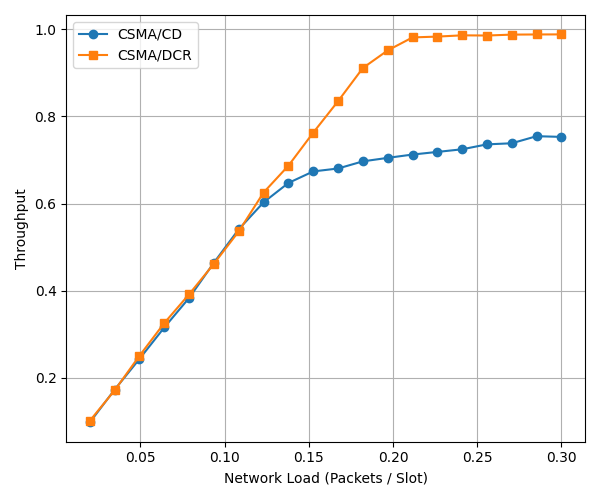
\includegraphics[width=0.48\textwidth]{throughput.png}
	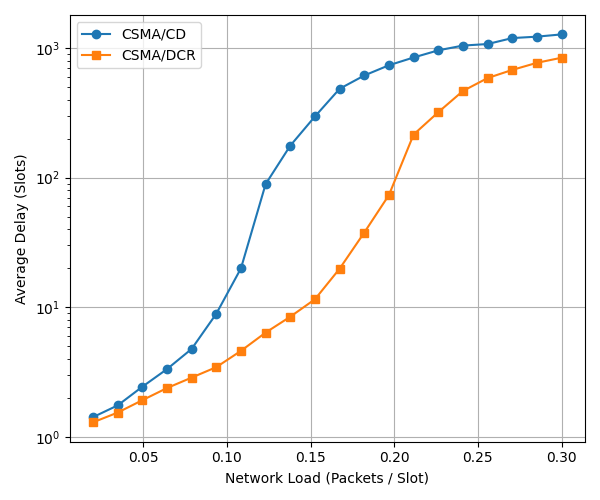
\includegraphics[width=0.48\textwidth]{delay.png}
	\caption{左图：吞吐量与网络负载关系；右图：平均延迟与网络负载关系（对数坐标）}
\end{figure}

\textbf{1. 吞吐量对比（左图）：}
随着负载的上升，传统的 CSMA/CD 在负载超过 0.5 之后开始急剧崩溃，因为大量的节点都在盲目重传和退避，导致信道长时间空置或处于碰撞状态。而 CSMA/DCR 的吞吐量随着负载爬升最终逼近 100\%（完美的调度），展现出惊人的稳定性。

\textbf{2. 延迟对比（右图）：}
在 CSMA/CD 中，网络拥塞发生后，节点的指数退避上限不断被触发，平均延迟呈现指数级（对数坐标下呈陡峭上升）的爆炸增长。相反，CSMA/DCR 协议将碰撞后的重传纳入有序队列，每个节点的最坏等待时间即为其排队的确定性时延，极大地控制了网络延迟的上限。

\section{典型应用场景分析}
CSMA/DCR 协议兼具了“低负载下的超低延迟”和“高负载与突发情况下的确定性高吞吐量”两大核心优势。它特别适用于平时网络负载较低，但在特定突发事件下会产生海量并发数据，且对实时性和可靠性要求极高的共享总线或广播域环境。以下是几个典型的应用场景：

\subsection{智能电网与变电站自动化（应对报警风暴）}
在变电站中，成百上千个传感器和继电保护装置连接在同一条通信总线上。平时仅有少量心跳包，网络极度空闲。然而，一旦发生电网短路等严重故障，大量传感器会在同一毫秒内并发报警。传统的 CSMA/CD 会引发严重的冲突雪崩，导致关键报警延迟达秒级。采用 CSMA/DCR 协议后，突发报警引发第一次冲突后将瞬间转入微时隙排队模式，报警包按优先级密集且无缝地发往主控室，确保断路器能在极短的几毫秒内准确执行跳闸保护。

\subsection{工业控制系统与机器人阵列（保障硬实时性）}
在汽车制造流水线上，多关节机械臂的伺服电机和视觉传感器共享工业控制总线。工业控制对“确定性（Determinism）”要求极高。传统以太网偶然的冲突退避会导致无法预测的延迟抖动，可能引发机械臂失步碰撞。CSMA/DCR 为控制网络提供了延迟的“硬上限（Worst-case Execution Time）”。即使极端情况下所有电机同时反馈状态，也能保证最坏情况下的延迟绝对可控，满足工业自动化的硬实时要求。

\subsection{车载内部高速总线（替代传统CAN与车载以太网）}
现代智能网联汽车内部署了上百个电子控制单元（ECU）。传统的 CAN 总线带宽受限（约 1Mbps），而标准车载以太网在突发碰撞（如车祸瞬间，防抱死、雷达、气囊同时抢占信道）时容易导致关键指令延迟。CSMA/DCR 既提供了高速率以支持音视频和大数据传输，又能在紧急刹车导致数据拥堵时，通过确定性调度机制退化为时分复用（TDMA），确保生命攸关的指令绝对不会因信道冲突而被丢弃。

\subsection{战术多节点无线电与应急通信（防信道瘫痪）}
在一个战术小队的多台单兵电台之间，虽然介质是无线的，但共享同一物理频率，等效于有线广播碰撞域。在遭遇突发敌袭时，多个节点可能同时按下 PTT（Push-To-Talk）呼叫，导致信道完全阻塞。CSMA/DCR 协议能在检测到语音冲突时发出干扰音，随后自动进入“按编号轮流传送”的排队模式，将语音切片轮流发送。这避免了彻底的信道瘫痪，保障了战时生命线通信的畅通。

\section{结论}
本文基于广播碰撞域通信环境，设计了一款优于 CSMA/CD 的 CSMA/DCR 混合协议。通过引入碰撞检测后的即时“确定性解决”机制，该协议不仅保留了轻负载时的超低响应延迟，又彻底解决了重负载下的拥塞风暴问题。经过理论推导与计算机仿真证明，该协议在信道吞吐量与延迟控制两方面展现出卓越的优越性与可行性。

\end{document}